\chapter{Conclusion} \label{chapter6}

    This application uses production-ready systems and tools for offering stability and scalability, as previously described in chapter \ref{chapter5}. It contains various modules designed to provide ease of use, transparency, and a structured data set.
    
\section{Results} \label{6:results}

    We published the application on \textbf{Google Play}\footnote{https://play.google.com/store/apps/details?id=ro.pub.acs.acs\_upb\_mobile} in March 2021. This represented a significant step both from the perspective of the development process and in terms of advertising. Before this date, users had to manually download and install the application \textit{\acrshort{apk}} installation file from our GitHub repository. Undoubtedly, this aspect was a significant disadvantage for our users for several reasons: lack of reliability and complicated installation method.
    
    After about three and a half months later, at the end of June 2021, our application has gathered more than \textbf{140} Play Store downloads and \textbf{17} \textit{5-stars} ratings. In addition, according to Firebase Analytics, more than \textbf{300} students have already registered their accounts, and more than \textbf{100} students are actively using our solution, as can be observed in figure \ref{6:fig:active_users}. On average, the application benefits from approximately three daily users, especially on Android devices. 
    
    \clearpage
    
    \begin{figure}[ht]
        \centering
             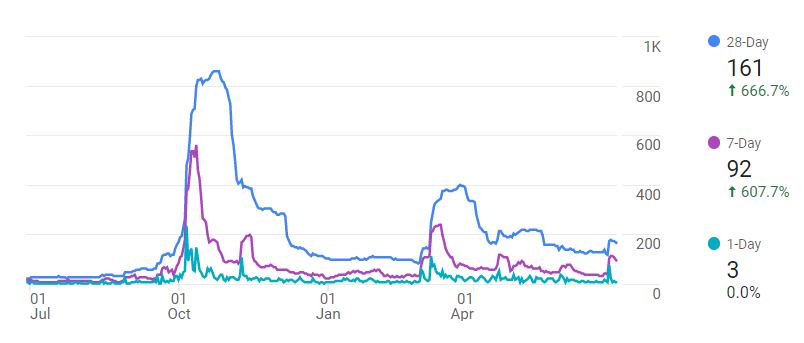
\includegraphics[height=0.25\textheight]{figures/charts/active_users.png}
        \caption{Active users, according to Firebase, plotted over the last \textbf{12} months}
        \label{6:fig:active_users}
    \end{figure}
    
    Students proved that they are generally delighted with the experience offered by this application. They shared with us appreciations about the people page and claimed that it frequently helped them quickly search for the contact details of a teacher. Moreover, some students mentioned that the feedback form has a catchy design, mainly thanks to the Likert scale questions, whose responses are represented by emoticons.
    
    We have already started to collect real answers from users in our production environment based on the feedback form implemented. Equally, we noticed a greater interest in using this feature among first-year students. This represents a gratifying aspect and demonstrates that students are eager to help each other with advice on the subjects studied.
    
    Although the application received overall positive feedback from users, we were suggested different ideas for enhancement. Thus, students expressed their desire to see in the timetable the periods when feedback questionnaires are enabled, just like vacations or exam sessions. Furthermore, we were advised to split the feedback form into multiple pages since it is pretty long. In the same manner, this modification would aid in better organization of the questions, and the \acrshort{ui} will be airier.
    
    On the statistics side, we received recommendations from students to display results for a specific series, specialization, or study program. Thus, students could find out general information more quickly without exploring the reviews of each class independently.

\section{Future improvements} \label{6:improvements}

    Although our application offers multiple functionalities even in the current stage, there are still many ideas that we will focus on further developing.
    
    \subsection{Gamification} \label{6:gamification}
    
    Gamification is a recently introduced concept that favors a more interactive and pleasant experience among users. According to a study performed in 2017 by Christo Dichev and Darina Dicheva \cite{dichev2017gamification}, this feature might have a significant impact on the educational environment by increasing the motivation of students to contribute to the well-being of this application. Thus, students will be rewarded with experience points as long as they add or complete various details from the application, like events in the timetable or feedback forms. Students will increase their level based on the points earned and receive specific badges or symbolic nicknames like modern games.
    
    Likewise, we plan to implement a globally visible leaderboard, highlighting the most active users and benefitting their competitiveness. As a result, the higher the score accumulated is, the more permissions students will receive in the application.
    
    Naturally, this module must also allow the discouragement of malicious students by decreasing their scores in case of intentionally adding erroneous or offensive information. In the worst-case scenario, this module should be capable of automatically retrieving access to our resources for students who lamentably violate the content of this application.
    
    \subsection{Filtering} \label{6:filtering}
    
    Since about a third of all questions from our questionnaire are open-ended, we offer students a high degree of freedom to express their thoughts. Nonetheless, although the purpose of our application is to encourage constructive feedback from students, we cannot completely prevent users from sharing their frustration through offensive comments.
    
    Even though we cannot guarantee an ideal environment with our solution, we intend to approach an optimal model. Therefore, to ensure that no inappropriate opinions are introduced in the application, we plan to integrate a feature that allows filtering the reviews offered by students.
    
    Perspective \acrshort{api}\footnote{https://www.perspectiveapi.com/} represents a suitable example in this respect. This framework calculates a threshold for each message, based on which we can establish a degree of toxicity. When the threshold is exceeded, the comment identified as offensive will be automatically excluded from our application. Thus, we ensure our users high-quality information by blocking any harmful words.
    
    This idea of filtering negative comments uses a \textbf{Machine Learning} (\acrshort{ml}) model, and the \acrshort{api}\footnote{https://developers.perspectiveapi.com/s/about-the-api} provided is hosted on Google Cloud Platform\footnote{https://cloud.google.com/}. We need to create a Firebase Cloud Function\footnote{https://firebase.google.com/docs/functions} which evaluates each comment added in the \textbf{\textit{forms}} collection and marks it as appropriate or not. Hence, we expect a relatively straightforward implementation of this feature.

\section{Mentorship} \label{6:mentorship}

    We are constantly trying to expand our team and encourage students to contribute as much as possible to the development of this open-source project. As a result, we decided to post an unpaid recruitment ad on a well-recognized platform for offering internships to students, called SPB\footnote{https://stagiipebune.ro/home/}. After about a month, our announcement caught the attention of over \textbf{100} students from different universities. Since this is a rather considerable number, we organized a recruitment process and interviewed the most suitable candidates that could deal with the future functionalities presented in section \ref{6:improvements} and beyond.
    
    Finally, we succeeded in finding \textbf{15} students who have demonstrated that they are interested and willing to continue implementing this project. They asked us pertinent questions regarding the structure of the project and the methods used for storing all the data. A mentor from our initial team will guide each newcomer. Thus, we promote the idea of making students more responsible and facilitate collaboration between them. Likewise, our project simulates a work environment similar to an official company in the \acrshort{itc} industry.
